\chapter{Gravitational Redshift, Tensors, and the Metric}

\section{What Gravity Does to a Vertical Light Ray}

We return to the elevator and turn the light ray through ninety degrees. A
bullet fired upward loses kinetic energy as it rises and therefore slows
down. Light cannot behave in quite that way. Every local observer measures
its speed to be \(c\), so the quantity that changes as the ray climbs is its
frequency. Upward propagation produces a redshift; downward propagation
produces a blueshift.

The accelerating elevator gives the quickest derivation. Let the elevator
be momentarily at rest when a photon is emitted from its roof toward the
floor. During the light-travel time the elevator accelerates upward. The
floor therefore moves toward the arriving photon, and the detector sees a
Doppler blueshift.

If the elevator height is \(h\), then to first order
\begin{equation}
  \Delta t \simeq \frac{h}{c},
  \qquad
  \Delta v \simeq g\Delta t \simeq \frac{gh}{c}.
  \label{eq:l03-travel-time}
\end{equation}
The first-order Doppler shift is consequently
\begin{equation}
  \frac{\Delta\nu}{\nu}
  \simeq
  \frac{\Delta v}{c}
  \simeq
  \frac{gh}{c^{2}}.
  \label{eq:l03-weak-redshift}
\end{equation}
For a downward ray this quantity is positive. Reversing the experiment
reverses the sign:
\begin{equation}
  \frac{\nu_{\mathrm{floor}}}{\nu_{\mathrm{roof}}}
  \simeq 1+\frac{gh}{c^{2}},
  \qquad
  \frac{\nu_{\mathrm{roof}}}{\nu_{\mathrm{floor}}}
  \simeq 1-\frac{gh}{c^{2}}.
  \label{eq:l03-up-down-shifts}
\end{equation}

\begin{figure}[tbp]
  \centering
  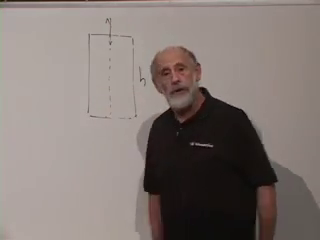
\includegraphics[width=0.72\textwidth]{lecture_03_figure_01.png}
  \caption{The vertical-light experiment in an elevator of height \(h\).
  During the photon's flight, upward acceleration changes the velocity of
  the receiving end of the elevator.}
  \lectureframe{00:05:00}
\end{figure}

\begin{classroomqa}
\audiencequestion{Why do the Doppler shifts not cancel as they would for
source and receiver moving together?
\lecturetimestamp{00:02:23--00:04:55}}
\lecturerresponse{A constant-velocity elevator has one inertial rest frame,
and source and receiver remain at rest in it. Here emission and reception
occur at different times while the elevator is accelerating. The source is
momentarily at rest at emission, but the receiver has acquired velocity by
reception. That change of velocity is precisely what survives in
Eq.~\eqref{eq:l03-weak-redshift}.}
\end{classroomqa}

The equivalence principle now turns the kinematic result into a
gravitational one. A laboratory supported in a uniform gravitational field
is locally equivalent to the upward-accelerating elevator. Light sent
downward is therefore blueshifted, while light sent upward is redshifted.
The effect is small near Earth, but it is measurable in a sufficiently
sensitive tower experiment.

The same reasoning applies to light escaping from the Sun. Its spectral
lines arrive redshifted relative to identical lines measured in the
laboratory. For a spherical source of mass \(M\) and radius \(R\), the weak
field scale is
\begin{equation}
  z
  \equiv
  \frac{\nu_{\mathrm{emit}}-\nu_{\mathrm{receive}}}
       {\nu_{\mathrm{receive}}}
  \simeq
  \frac{GM}{Rc^{2}}
  =
  \frac{v_{\mathrm{esc}}^{2}}{2c^{2}}.
  \label{eq:l03-compactness}
\end{equation}
Large radius alone is not decisive. What matters is compactness, or
equivalently the escape speed. White dwarfs and neutron stars produce
larger shifts than ordinary stars, and the redshift becomes extreme near a
black-hole horizon.

\begin{classroomqa}
\audiencequestion{Would a physically larger star necessarily produce a
larger redshift?
\lecturetimestamp{00:06:00--00:07:35}}
\lecturerresponse{Not necessarily. The controlling dimensionless
combination is \(GM/(Rc^{2})\), not \(M\) or \(R\) separately. A compact
object can have a much larger surface redshift than a more massive but
diffuse object.}
\end{classroomqa}

\begin{classroomqa}
\audiencequestion{Does the frequency shift contradict the equivalence
principle by revealing gravity inside the elevator?
\lecturetimestamp{00:08:30--00:09:22}}
\lecturerresponse{No. The supported elevator is equivalent to an
accelerated laboratory, not to an inertial one. The shift is the same
observable described either as a Doppler effect in the accelerating frame
or as a gravitational frequency shift in the supported laboratory.}
\end{classroomqa}

\section{Free Fall and the Local Disappearance of Gravity}

Now release the elevator. Send a photon downward while the entire laboratory
falls. Relative to observers held fixed in the gravitational field, the
photon gains frequency as it descends. At the same time the floor falls away
from the photon and produces an opposing kinematic redshift. In a
sufficiently small freely falling laboratory the two effects cancel:
\begin{equation}
  \left(\frac{\Delta\nu}{\nu}\right)_{\mathrm{grav}}
  +
  \left(\frac{\Delta\nu}{\nu}\right)_{\mathrm{Doppler}}
  =0.
  \label{eq:l03-freefall-cancellation}
\end{equation}
An exact calculation must use special-relativistic Doppler factors. A
Newtonian expansion establishes the leading cancellation but can leave
spurious higher-order terms. The exact local cancellation is what the
equivalence principle requires.

\begin{figure}[tbp]
  \centering
  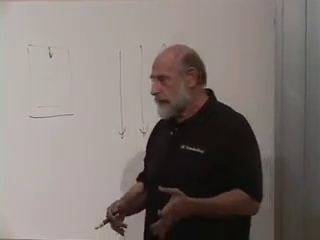
\includegraphics[width=0.78\textwidth]{lecture_03_figure_02.png}
  \caption{The freely falling elevator. Gravitational blueshift of the
  descending light and the receiver's kinematic redshift cancel in the
  local experiment.}
  \lectureframe{00:12:05}
\end{figure}

\begin{classroomqa}
\audiencequestion{Why should a falling detector see no net shift when both
the photon and the elevator are accelerating?
\lecturetimestamp{00:09:22--00:12:48}}
\lecturerresponse{The two accelerations enter differently. Relative to a
supported frame, gravity blueshifts the downward photon, while the falling
floor moves away from it and redshifts the received signal. In the local
freely falling frame these are not two independent effects; they are the
two descriptions whose cancellation makes that frame locally inertial.
Only variations of gravity across the apparatus can remain.}
\end{classroomqa}

This qualification, \emph{locally}, is essential. A uniform acceleration
can be absorbed into the coordinates used to describe a small laboratory.
In an inertial picture, the meter sticks fixed in an accelerating elevator
trace a family of curved trajectories. The resulting coordinate grid is
curved even though the underlying spacetime used in this preliminary
argument is flat.

\begin{figure}[tbp]
  \centering
  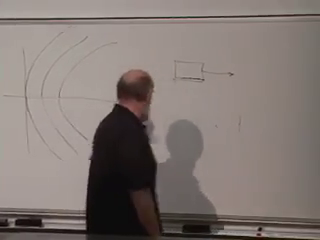
\includegraphics[width=0.78\textwidth]{lecture_03_figure_03.png}
  \caption{Curved trajectories traced by the meter sticks of an accelerating
  coordinate system. Apparent gravity can arise from the coordinates even
  when the underlying geometry is flat.}
  \lectureframe{00:14:25}
\end{figure}

The field of a real gravitating body is not uniform over an extended region.
Its direction changes from place to place, and its strength changes with
distance. One freely falling elevator can match the field near one chosen
trajectory, but no single elevator removes the field everywhere. Neighboring
freely falling bodies acquire relative acceleration: the tidal effect.

\begin{figure}[tbp]
  \centering
  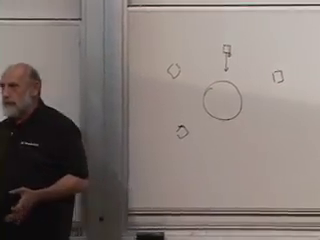
\includegraphics[width=0.76\textwidth]{lecture_03_figure_04.png}
  \caption{Several local laboratories around a gravitating body. Their
  acceleration directions differ, displaying why one global accelerated
  frame cannot remove the whole field.}
  \lectureframe{00:17:40}
\end{figure}

\begin{classroomqa}
\audiencequestion{Is this already the Rindler coordinate construction?
\lecturetimestamp{00:18:00--00:18:55}}
\lecturerresponse{It is the same physical direction, but the present
discussion is deliberately pre-relativistic. The exact Rindler chart
requires special relativity and will be treated only after the geometric
language is in place.}
\end{classroomqa}

We have therefore reached the first geometric statement of general
relativity. Gravity that is common to an infinitesimal freely falling
laboratory can be transformed away. Tidal gravity cannot. The obstruction
to removing the latter will become the curvature of spacetime. To describe
that obstruction without tying ourselves to one coordinate grid, we need
tensor calculus.

\section{Coordinates, Scalars, and Infinitesimal Changes}

Begin with ordinary \(d\)-dimensional space, before adding time. Label a
point by
\begin{equation}
  x=(x^{1},x^{2},\ldots,x^{d}),
\end{equation}
and let \(\phi_{(x)}(x)\) be a scalar field. An infinitesimal displacement
has coordinate components \(dx^{1},\ldots,dx^{d}\). The corresponding change
of the scalar is its total differential,
\begin{equation}
  d\phi
  =
  \sum_{m=1}^{d}
  \frac{\partial\phi}{\partial x^{m}}\,dx^{m}.
  \label{eq:l03-total-differential-sum}
\end{equation}

\begin{figure}[tbp]
  \centering
  
\includegraphics[width=0.80\textwidth]{lecture_03_figure_05.png}
  \caption{A \(d\)-dimensional coordinate system, a scalar field
  \(\phi(x)\), and the infinitesimal displacement \(dx\) used in the total
  differential.}
  \lectureframe{00:23:00}
\end{figure}

From now on a repeated index is summed unless stated otherwise. With this
Einstein convention,
\begin{equation}
  \boxed{
  d\phi
  =
  \frac{\partial\phi}{\partial x^{m}}\,dx^{m}.}
  \label{eq:l03-total-differential}
\end{equation}
The repeated \(m\) is a dummy index. Renaming it \(r\) changes nothing,
provided the same label is used in both factors and does not collide with a
free index.

\begin{figure}[tbp]
  \centering
  
\includegraphics[width=0.80\textwidth]{lecture_03_figure_06.png}
  \caption{The total differential written first as an explicit sum and then
  in the repeated-index convention.}
  \lectureframe{00:25:40}
\end{figure}

\begin{classroomqa}
\audiencequestion{Does the order of the differentials matter, and is
\(d\phi\) a finite change?
\lecturetimestamp{00:27:30--00:30:08}}
\lecturerresponse{The components here are ordinary commuting numbers, so
their products commute. The symbol \(d\) denotes the first-order
differential. For a finite displacement \(\Delta x\), higher-order terms
generally enter; Eq.~\eqref{eq:l03-total-differential} is the linear
infinitesimal relation.}
\end{classroomqa}

Introduce another coordinate system,
\begin{equation}
  y^{n}=y^{n}(x^{1},\ldots,x^{d}).
  \label{eq:l03-coordinate-map}
\end{equation}
An admissible change of coordinates is one-to-one on the region being used,
differentiable, and equipped with a differentiable inverse. It relabels
points; it does not change the dimension of the space. The chain rule gives
\begin{equation}
  \boxed{
  \frac{\partial\phi}{\partial y^{n}}
  =
  \frac{\partial\phi}{\partial x^{m}}
  \frac{\partial x^{m}}{\partial y^{n}}.}
  \label{eq:l03-chain-rule}
\end{equation}
For each free index \(n\), the repeated index \(m\) is summed.

\begin{figure}[tbp]
  \centering
  
\includegraphics[width=0.82\textwidth]{lecture_03_figure_07.png}
  \caption{The scalar chain rule between the \(x\) and \(y\) coordinate
  systems. The repeated index \(m\) is summed while \(n\) remains free.}
  \lectureframe{00:35:05}
\end{figure}

The direct and inverse Jacobians satisfy
\begin{equation}
  \frac{\partial x^{m}}{\partial y^{n}}
  \frac{\partial y^{n}}{\partial x^{r}}
  =
  \delta^{m}{}_{r}.
  \label{eq:l03-inverse-jacobians}
\end{equation}
This identity is the coordinate version of multiplying a nonsingular matrix
by its inverse.

\begin{classroomqa}
\audiencequestion{What restrictions are imposed on a coordinate
transformation?
\lecturetimestamp{00:30:08--00:31:48}}
\lecturerresponse{Within the region under discussion, each point must have
a unique label and the map must be smooth enough to differentiate. Its
Jacobian must be nonsingular so that the inverse coordinates exist. A chart
may fail at a boundary or coordinate singularity, but it must be regular
where the tensor formulas are used.}
\end{classroomqa}

\begin{classroomqa}
\audiencequestion{Can a coordinate change alter the number of coordinates?
\lecturetimestamp{00:37:45--00:38:55}}
\lecturerresponse{No. Both charts describe the same \(d\)-dimensional
space. They have the same number of independent coordinates, and the
inverse transformation returns one set from the other.}
\end{classroomqa}

\section{Geometric Objects and Their Components}

Draw two grids on the same plane, one rectangular and one skew. The points,
curves, and arrows in the plane have not changed, but their numerical
coordinates have. Tensor notation separates the geometric object from the
components used to represent it.

\begin{figure}[tbp]
  \centering
  
\includegraphics[width=0.78\textwidth]{lecture_03_figure_08.png}
  \caption{Two coordinate grids on the same plane. The red skew grid changes
  component values without changing the geometric objects being described.}
  \lectureframe{00:40:10}
\end{figure}

A scalar is the simplest example. It assigns one coordinate-independent
number to each point. If \(x\) and \(y\) label the same point, the two
coordinate representations obey
\begin{equation}
  \phi_{(y)}(y)
  =
  \phi_{(x)}(x(y)).
  \label{eq:l03-scalar-invariance}
\end{equation}
This is what it means to call a scalar a rank-zero tensor.

\begin{figure}[tbp]
  \centering
  
\includegraphics[width=0.82\textwidth]{lecture_03_figure_09.png}
  \caption{Scalar invariance and a free displacement vector. The scalar has
  the same value at the same point, while vector components change with the
  coordinate grid.}
  \lectureframe{00:47:30}
\end{figure}

The infinitesimal displacement is the model contravariant vector. Applying
the total-differential rule to each coordinate function \(y^{n}(x)\) gives
\begin{equation}
  dy^{n}
  =
  \frac{\partial y^{n}}{\partial x^{m}}\,dx^{m}.
  \label{eq:l03-displacement-law}
\end{equation}
Any contravariant vector transforms by the same rule:
\begin{equation}
  \boxed{
  V_{(y)}^{n}
  =
  \frac{\partial y^{n}}{\partial x^{m}}\,V_{(x)}^{m}.}
  \label{eq:l03-contravariant-vector}
\end{equation}

\begin{figure}[tbp]
  \centering
  
\includegraphics[width=0.84\textwidth]{lecture_03_figure_10.png}
  \caption{The displacement law and the general contravariant-vector
  transformation. The Jacobian converts \(x\)-components into
  \(y\)-components.}
  \lectureframe{00:51:15}
\end{figure}

\begin{classroomqa}
\audiencequestion{What is contravariant about a contravariant vector?
\lecturetimestamp{00:51:25--00:52:36}}
\lecturerresponse{The name refers to its transformation behavior. Its
components transform with the direct Jacobian
\(\partial y/\partial x\), whereas gradients and other covectors transform
with the inverse Jacobian \(\partial x/\partial y\). The distinction is
encoded by upper and lower indices.}
\end{classroomqa}

\section{Higher-Rank Tensors and Covectors}

If \(A^{m}\) and \(B^{n}\) are contravariant vectors, their component
products provide a rank-two example,
\begin{equation}
  T^{mn}=A^{m}B^{n}.
\end{equation}
There are \(d^{2}\) components, and each upper index brings its own direct
Jacobian:
\begin{equation}
  \boxed{
  T_{(y)}^{pq}
  =
  \frac{\partial y^{p}}{\partial x^{m}}
  \frac{\partial y^{q}}{\partial x^{n}}
  T_{(x)}^{mn}.}
  \label{eq:l03-rank-two-contravariant}
\end{equation}
Not every rank-two tensor need be a single product of two vectors; the
product is a convenient way to discover the transformation pattern.

\begin{figure}[tbp]
  \centering
  
\includegraphics[width=0.84\textwidth]{lecture_03_figure_11.png}
  \caption{The rank-two contravariant transformation law. Each upper index
  contributes one factor of the direct Jacobian.}
  \lectureframe{00:59:40}
\end{figure}

\begin{classroomqa}
\audiencequestion{What assumptions are hidden in this manipulation?
\lecturetimestamp{01:00:00--01:03:12}}
\lecturerresponse{The components are ordinary numbers, so multiplication
commutes. The coordinate functions are differentiable, and the Jacobian is
invertible because the coordinate map is locally one-to-one. These are the
same regularity assumptions already used in the chain rule.}
\end{classroomqa}

The gradient of a scalar transforms oppositely. Define
\begin{equation}
  A_{m}^{(x)}
  =
  \frac{\partial\phi}{\partial x^{m}}.
\end{equation}
Equation~\eqref{eq:l03-chain-rule} says
\begin{equation}
  \boxed{
  A_{n}^{(y)}
  =
  \frac{\partial x^{m}}{\partial y^{n}}\,A_{m}^{(x)}.}
  \label{eq:l03-covector}
\end{equation}
This is a covariant vector, or covector. Contravariant components carry
upper indices; covariant components carry lower indices.

\begin{figure}[tbp]
  \centering
  
\includegraphics[width=0.84\textwidth]{lecture_03_figure_12.png}
  \caption{Contravariant and covariant vector laws displayed together. The
  direct and inverse Jacobians explain the upper- and lower-index notation.}
  \lectureframe{01:07:40}
\end{figure}

An upper index can be contracted with a lower index:
\begin{equation}
  A_{n}V^{n}.
  \label{eq:l03-contraction}
\end{equation}
Under a coordinate transformation the two Jacobians cancel by
Eq.~\eqref{eq:l03-inverse-jacobians}, leaving a scalar. This is why the
placement of indices is more than typography.

With two lower indices the transformation rule is
\begin{equation}
  \boxed{
  T_{mn}^{(y)}
  =
  \frac{\partial x^{r}}{\partial y^{m}}
  \frac{\partial x^{s}}{\partial y^{n}}
  T_{rs}^{(x)}.}
  \label{eq:l03-rank-two-covariant}
\end{equation}

\begin{figure}[tbp]
  \centering
  
\includegraphics[width=0.84\textwidth]{lecture_03_figure_13.png}
  \caption{The rank-two covariant transformation law, with one inverse
  Jacobian for each lower index.}
  \lectureframe{01:11:45}
\end{figure}

\begin{classroomqa}
\audiencequestion{Are upper and lower indices merely names for two different
lists of numbers?
\lecturetimestamp{01:09:15--01:11:42}}
\lecturerresponse{They label two dual transformation laws. A vector and a
covector are different geometric kinds of object, although the metric will
soon provide a systematic map between them. The index placement also tells
us which contractions are coordinate invariant.}
\end{classroomqa}

\section{The Metric as a Tensor}

After the break, begin again with the most familiar geometry: Euclidean
space in Cartesian coordinates. For an infinitesimal displacement,
Pythagoras gives
\begin{equation}
  ds^{2}
  =
  (dx^{1})^{2}+(dx^{2})^{2}+\cdots+(dx^{d})^{2}.
  \label{eq:l03-pythagoras}
\end{equation}
The superscript on \(x^{m}\) labels a component; the superscript on
\(ds^{2}\) is an actual square. Introduce the Kronecker delta,
\begin{equation}
  \delta_{mn}
  =
  \begin{cases}
    1, & m=n,\\
    0, & m\ne n,
  \end{cases}
\end{equation}
and write
\begin{equation}
  \boxed{
  ds^{2}
  =
  \delta_{mn}\,dx^{m}dx^{n}.}
  \label{eq:l03-cartesian-metric}
\end{equation}

\begin{figure}[tbp]
  \centering
  
\includegraphics[width=0.84\textwidth]{lecture_03_figure_14.png}
  \caption{Pythagoras and the Kronecker-delta form of the Cartesian line
  element. The metric measures the squared length of an infinitesimal
  displacement.}
  \lectureframe{01:22:20}
\end{figure}

Now change from \(x\) to \(y\). The differentials obey
\begin{equation}
  dx^{m}
  =
  \frac{\partial x^{m}}{\partial y^{r}}\,dy^{r}.
\end{equation}
Substitution into Eq.~\eqref{eq:l03-cartesian-metric} gives
\begin{align}
  ds^{2}
  &=
  \delta_{mn}
  \frac{\partial x^{m}}{\partial y^{r}}
  \frac{\partial x^{n}}{\partial y^{s}}
  dy^{r}dy^{s}
  \nonumber\\
  &=
  g_{rs}^{(y)}(y)\,dy^{r}dy^{s},
  \label{eq:l03-transformed-line-element}
\end{align}
where
\begin{equation}
  \boxed{
  g_{rs}^{(y)}(y)
  =
  \delta_{mn}
  \frac{\partial x^{m}}{\partial y^{r}}
  \frac{\partial x^{n}}{\partial y^{s}}.}
  \label{eq:l03-metric-from-cartesian}
\end{equation}

\begin{figure}[tbp]
  \centering
  
\includegraphics[width=0.86\textwidth]{lecture_03_figure_15.png}
  \caption{The Cartesian line element transformed to arbitrary coordinates.
  The circled coefficient is the metric \(g_{rs}^{(y)}\).}
  \lectureframe{01:28:10}
\end{figure}

More generally, if the metric in the \(x\)-coordinates is
\(g_{mn}^{(x)}\), then
\begin{equation}
  \boxed{
  g_{rs}^{(y)}
  =
  g_{mn}^{(x)}
  \frac{\partial x^{m}}{\partial y^{r}}
  \frac{\partial x^{n}}{\partial y^{s}}.}
  \label{eq:l03-general-metric-transform}
\end{equation}
The metric is therefore a rank-two covariant tensor. The number \(ds^{2}\)
is invariant, while the components \(g_{mn}\) and \(dx^{m}\) change in
compensating ways.

\section{Flat Space, Curved Space, and Local Coordinates}

A space is flat on a region if coordinates can be found throughout that
region in which
\begin{equation}
  g_{mn}=\delta_{mn}.
  \label{eq:l03-flatness}
\end{equation}
Complicated, position-dependent metric components do not by themselves
prove curvature; they may arise from curvilinear coordinates on a flat
space. Curvature is the obstruction to transforming the metric to the
Cartesian form over the region under consideration.

\begin{classroomqa}
\audiencequestion{So is flatness exactly the existence of coordinates that
reduce the metric to \(\delta_{mn}\)?
\lecturetimestamp{01:31:20--01:34:22}}
\lecturerresponse{Yes, provided the region is specified. Flatness means
that one coordinate transformation works throughout that region. A metric
that merely looks complicated in the current chart may still describe flat
space.}
\end{classroomqa}

At any regular point of a smooth Riemannian geometry, coordinates can be
chosen so that the metric equals \(\delta_{mn}\) at that point, and even so
that its first derivatives vanish there. This is a pointwise statement, not
a claim that a finite neighborhood is exactly Euclidean. Curvature appears
in the second-order departure from that locally Cartesian form.

The cone is a useful warning about local and global statements. Away from
its tip, a small patch can be cut and unrolled into the plane, so its
intrinsic geometry is locally flat. At the tip there is a conical
singularity, and globally the missing or excess angle cannot be removed by
one smooth Cartesian chart.

\begin{figure}[tbp]
  \centering
  
\includegraphics[width=0.78\textwidth]{lecture_03_figure_16.png}
  \caption{A cone and a locally flattened patch. The construction separates
  pointwise or local flatness from a global obstruction concentrated at the
  cone's tip.}
  \lectureframe{01:36:40}
\end{figure}

\begin{classroomqa}
\audiencequestion{Can the metric always be made Euclidean in a sufficiently
small neighborhood?
\lecturetimestamp{01:34:22--01:37:18}}
\lecturerresponse{It can always be made Euclidean at one regular point.
Over a finite neighborhood, exact Euclidean form is possible only when the
curvature vanishes there. The cone is locally flat away from its tip, but a
genuinely curved surface such as a sphere retains second-order curvature in
every neighborhood.}
\end{classroomqa}

\section{Polar Coordinates in the Flat Plane}

Polar coordinates supply the decisive example of a nonconstant metric in a
flat space:
\begin{equation}
  x=r\cos\theta,
  \qquad
  y=r\sin\theta.
  \label{eq:l03-polar-map}
\end{equation}
Differentiate:
\begin{align}
  dx &= \cos\theta\,dr-r\sin\theta\,d\theta,
  \nonumber\\
  dy &= \sin\theta\,dr+r\cos\theta\,d\theta.
  \label{eq:l03-polar-differentials}
\end{align}

\begin{figure}[tbp]
  \centering
  
\includegraphics[width=0.84\textwidth]{lecture_03_figure_17.png}
  \caption{The Cartesian-to-polar map and its differential form. These
  relations are substituted directly into \(dx^{2}+dy^{2}\).}
  \lectureframe{01:41:55}
\end{figure}

Substituting and expanding,
\begin{align}
  ds^{2}
  &=
  dx^{2}+dy^{2}
  \nonumber\\
  &=
  \bigl(\cos\theta\,dr-r\sin\theta\,d\theta\bigr)^{2}
  +
  \bigl(\sin\theta\,dr+r\cos\theta\,d\theta\bigr)^{2}
  \nonumber\\
  &=
  dr^{2}+r^{2}d\theta^{2}.
  \label{eq:l03-polar-line-element}
\end{align}
The mixed terms cancel. Thus
\begin{equation}
  (g_{ab})
  =
  \begin{pmatrix}
    g_{rr} & g_{r\theta}\\
    g_{\theta r} & g_{\theta\theta}
  \end{pmatrix}
  =
  \begin{pmatrix}
    1 & 0\\
    0 & r^{2}
  \end{pmatrix}.
  \label{eq:l03-polar-metric}
\end{equation}

\begin{figure}[tbp]
  \centering
  
\includegraphics[width=0.84\textwidth]{lecture_03_figure_18.png}
  \caption{The completed polar-coordinate metric:
  \(g_{rr}=1\), \(g_{r\theta}=0\), and
  \(g_{\theta\theta}=r^{2}\).}
  \lectureframe{01:45:45}
\end{figure}

\begin{classroomqa}
\audiencequestion{Does the vanishing off-diagonal term prove that the plane
is flat?
\lecturetimestamp{01:45:15--01:47:05}}
\lecturerresponse{No. It says that the \(r\)- and \(\theta\)-coordinate
curves meet orthogonally. Diagonal form is useful, but curvature is a
different question. The plane is flat because the polar metric can be
transformed back to \(dx^{2}+dy^{2}\).}
\end{classroomqa}

\section{The Metric on a Sphere}

Finally take a unit sphere. Let \(\phi\) be the polar angle measured from
the north pole and let \(\theta\) be the azimuthal angle. A displacement in
the \(\phi\) direction has length \(d\phi\). At fixed \(\phi\), the circle
of latitude has radius \(\sin\phi\), so an azimuthal displacement has length
\(\sin\phi\,d\theta\). The two coordinate directions are orthogonal, and
\begin{equation}
  \boxed{
  ds^{2}
  =
  d\phi^{2}
  +
  \sin^{2}\phi\,d\theta^{2}.}
  \label{eq:l03-sphere-metric}
\end{equation}
For a sphere of radius \(R\), the right-hand side is multiplied by
\(R^{2}\).

\begin{figure}[tbp]
  \centering
  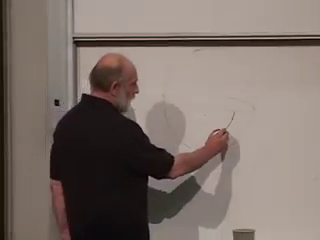
\includegraphics[width=0.78\textwidth]{lecture_03_figure_19.png}
  \caption{Polar and azimuthal displacements on a sphere. The shrinking
  latitude-circle radius supplies the factor \(\sin\phi\) in the metric.}
  \lectureframe{01:49:30}
\end{figure}

The polar metric of the plane and the angular metric of the sphere now look
similar, but they describe different intrinsic geometry. The plane's
position-dependent coefficient can be removed by returning to Cartesian
coordinates. The sphere's curvature cannot be removed over any finite
patch. This is the distinction needed for gravity: coordinates may create
apparent fields, but tidal effects reveal an invariant geometric
obstruction. The metric tensor is the object that carries that geometry
from one coordinate system to another.
